\documentclass[tikz,border=10pt]{standalone}
\begin{document}
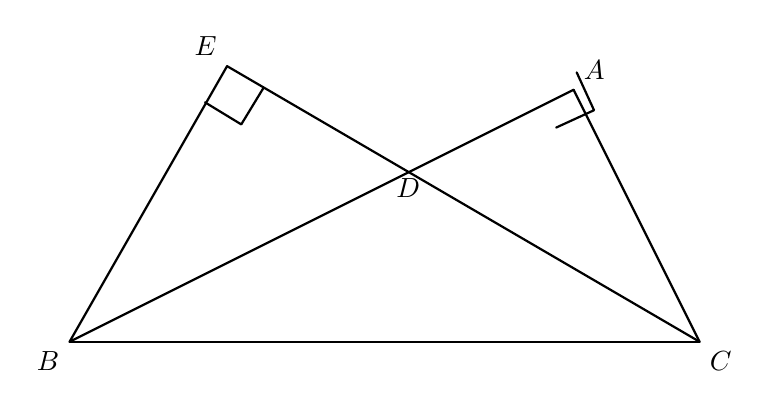
\begin{tikzpicture}[line cap=round,line join=round,thick]

\coordinate (B) at (0,0);
\coordinate (C) at (8,0);
\coordinate (E) at (2,3.5);
\coordinate (A) at (6.4,3.2);
\coordinate (D) at (4.3,2.2);

\draw (B) -- (C);
\draw (B) -- (E);
\draw (E) -- (C);
\draw (B) -- (A);
\draw (A) -- (C);

\draw (E) ++(-0.28,-0.46) -- ++(0.46,-0.28) -- ++(0.28,0.46);
\draw (A) ++(-0.22,-0.48) -- ++(0.48,0.22) -- ++(-0.22,0.48);

\node[below left] at (B) {$B$};
\node[below right] at (C) {$C$};
\node[above left] at (E) {$E$};
\node[above right] at (A) {$A$};
\node[below] at (D) {$D$};

\end{tikzpicture}
\end{document}
